
La~\cref{fig:Control-Diagrama UML de despliegue} define el diagrama UML de despliegue para el programa de control.
Este programa tiene acceso directo al hardware.
Ejecutará los comandos recibidos por el programa cliente y actuará en consecuencia sobre el motor de corriente continua.

\begin{figure}[H]
    \centering
    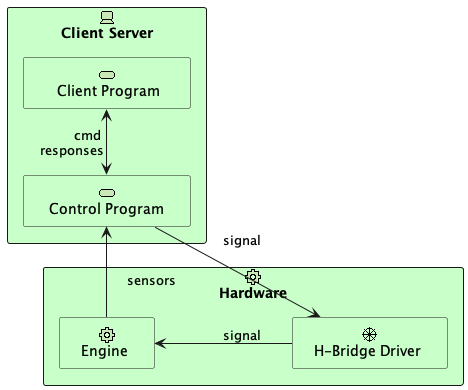
\includegraphics[height=0.35\textheight]{./part/Proyecto_ejecutivo/memoria_descriptiva/descripcionDelProyecto/control/uml/controlConcept}
    \caption{Control: Diagrama UML de despliegue}\label{fig:Control-Diagrama UML de despliegue}
\end{figure}

\subparagraph{Dominio}

\begin{itemize}
    \item PhysicModule: definición de variables físicas.
    Son interfaces de int y floats que garantizan la congruencia en las operaciones.
    Aunque los tipos sean float hay variables que no pueden operar entre sí sin atender a su realidad física, es decir sus unidades.
    \item PinModule: abstracción del sistema donde se ejecute el código.
    Dependerá del hardware necesario para atender a interfaz física de un motor
    \begin{itemize}
        \item EncoderPinModule: pin de entrada tipo pull para esperar a los flancos de subida del encoder.
        \item OutPinModule: pin de salida digital para activar o desactivar frenos y triggers de dirección.
        \item PWMPinModule: pin de control PWM con frecuencia y un ciclo de trabajo.
    \end{itemize}
    \item EncoderModule: \textit{Aggregate Root } compuesto por dos pines de tipo Encoder para leer los pulsos y calcular dirección y posición.
    \item EngineModule: interfaz del motor y la implementación.
    \item EnginePIDControllerModule: algoritmo de control PId.
    El controlador usará una instancia de Engine y una instancia de PIDAlgorithm
\end{itemize}


\begin{figure}[H]
    \centering
    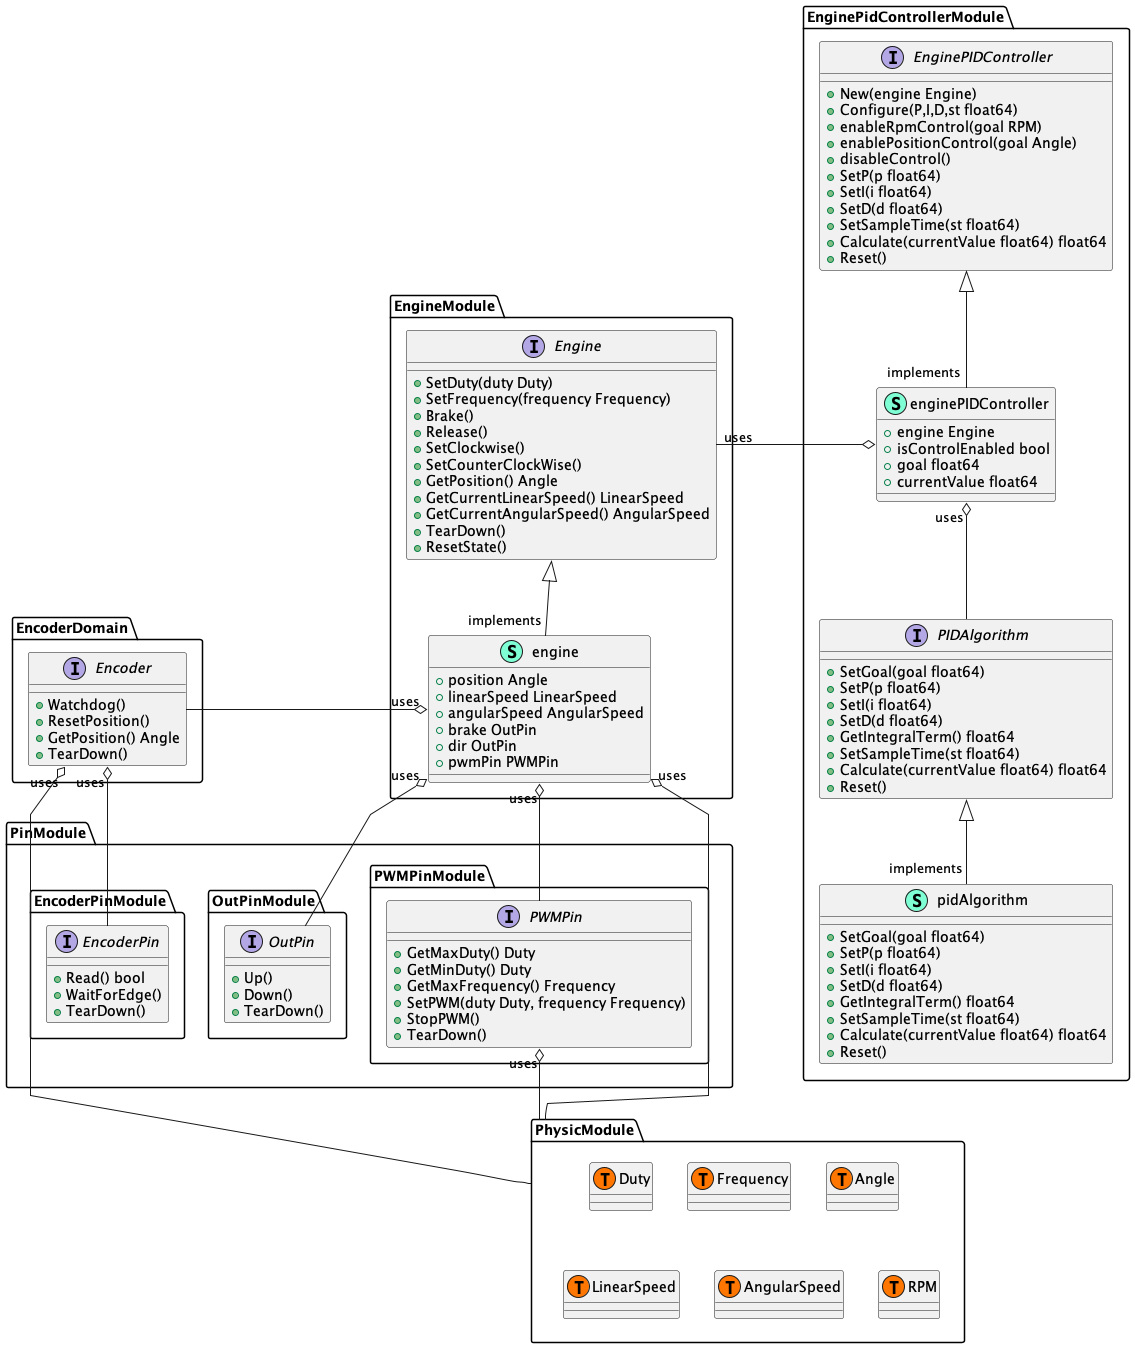
\includegraphics[height=0.6\textheight]{./part/Proyecto_ejecutivo/memoria_descriptiva/descripcionDelProyecto/control/uml/controlDomain}
    \caption{Control: Diagrama UML de el dominio}\label{fig:Control-Diagrama UML de el dominio}
\end{figure}

\subparagraph{Casos de uso}

Los casos de usos actuarán sobre el objeto de dominio \textit{EnginePIDController}.
Al no existir persistencia, y por lo tanto no necesitar identificadores, serán ValueObjects.
Particularmente el programa sólo instanciará uno.
No se hará uso de un patrón singleton ya a que podría desearse controlar varios motores a la vez en el futuro, Si el hardware lo permitiera.

\begin{itemize}
    \item \textbf{Configure PID}: El primer paso a ejecutar antes de habilitar el control PID será sintonizarlo.

    \begin{figure}[H]
        \centering
        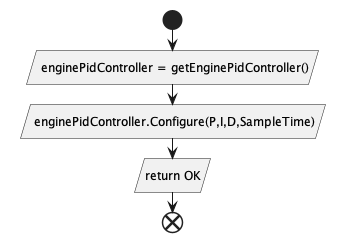
\includegraphics[height=0.2\textheight]{./part/Proyecto_ejecutivo/memoria_descriptiva/descripcionDelProyecto/control/uml/configurePID}
        \caption{Use Case: Configure PID}\label{fig:Use Case-Configure PID}
    \end{figure}

    \item \textbf{Disable control}

    \begin{figure}[H]
        \centering
        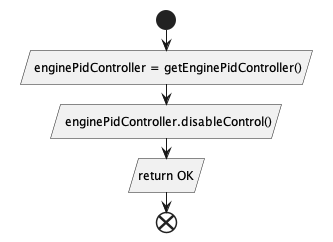
\includegraphics[height=0.2\textheight]{./part/Proyecto_ejecutivo/memoria_descriptiva/descripcionDelProyecto/control/uml/disableControl}
        \caption{Use Case: Disable control}\label{fig:Use Case- Disable control}
    \end{figure}

    \item \textbf{Enable RPM control}: Cuando se habilita el control rpm se genera una goRutine, es decir, si el hardware no devuelve error se responde OK pero un nuevo proceso que se quedará ejecutando hasta que se ejecute el caso de uso Disable Control.
    Este nuevo proceso ejecutará el control PID para mantener la consigna en el valor indicado.
    En este caso la consigna será la velocidad angular requerida.

    \begin{figure}[H]
        \centering
        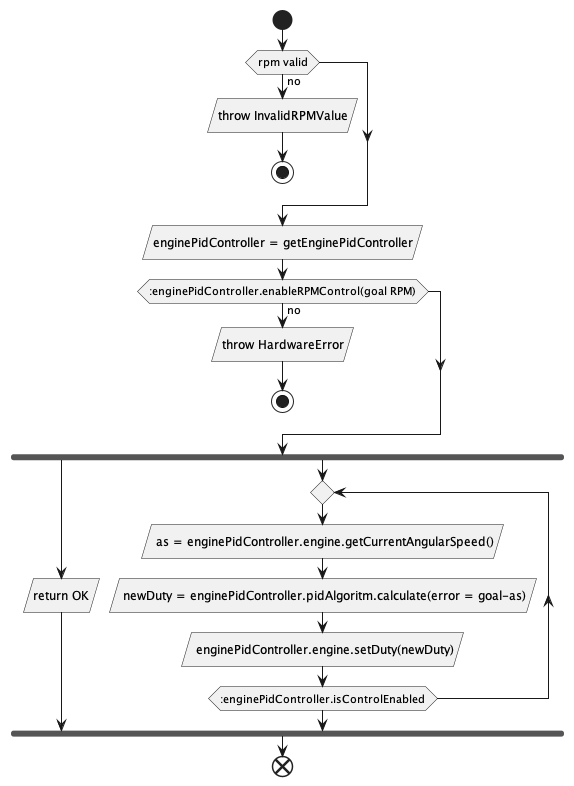
\includegraphics[height=0.6\textheight]{./part/Proyecto_ejecutivo/memoria_descriptiva/descripcionDelProyecto/control/uml/enableRPMControl}
        \caption{Use Case: Enable RPM control}\label{fig:Use Case- Enable RPM control}
    \end{figure}

    \item \textbf{Enable Position control}

    Para el control en posición se actuará análogamente al control de velocidad pero la consigna será el ángulo requerido.

    \begin{figure}[H]
        \centering
        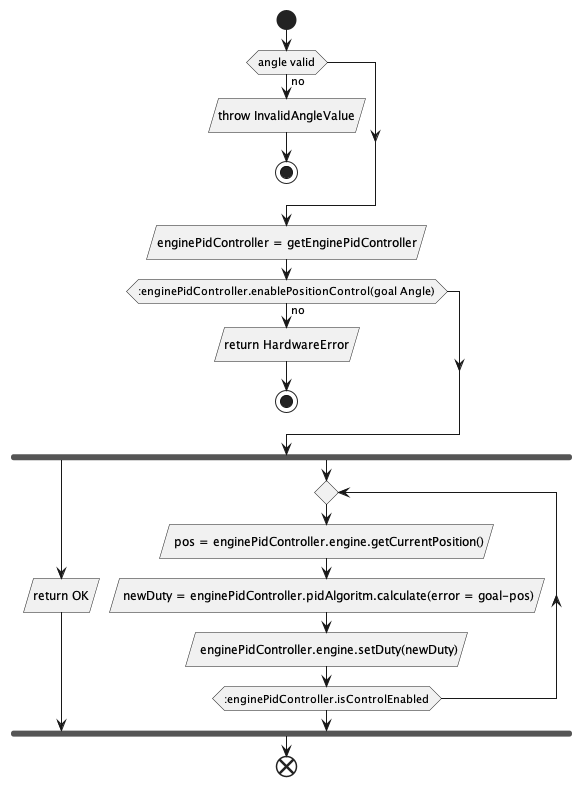
\includegraphics[height=0.4\textheight]{./part/Proyecto_ejecutivo/memoria_descriptiva/descripcionDelProyecto/control/uml/enablePositionControl}
        \caption{Use Case: Enable Position control}\label{fig:Use Case- Enable Position control}
    \end{figure}
\end{itemize}

\subparagraph{Estructura de carpetas}

\begin{figure}[H]
    \setlength{\DTbaselineskip}{10pt}
    \DTsetlength{0.2em}{1em}{0.2em}{0.4pt}{1.6pt}
    \dirtree{%
        .1 Project .
            .2 Domain.
            .2 Application.
            .2 Adapter.
            .2 Bootstrap.
    }
    \caption{Control: Estructura de carpetas de proyecto}\label{fig:Control- Estructura de carpetas de proyecto}
\end{figure}

\textbf{Dominio}

\begin{figure}[H]
    \setlength{\DTbaselineskip}{10pt}
    \DTsetlength{0.2em}{1em}{0.2em}{0.4pt}{1.6pt}
    \dirtree{%
        .1 Domain.
            .2 EnginePidController.
                .3 \textcolor{blue}{EnginePidController.go}.
                .3 Service.
                    .4 \textcolor{blue}{Configurator.go}.
                    .4 \textcolor{blue}{RPMControllerActivator.go}.
                    .4 \textcolor{blue}{PositionControllerActivator.go}.
                    .4 \textcolor{blue}{ControlDisabler.go}.
            .2 Engine.
                .3 \textcolor{blue}{EngineVo.go}.
                .3 Repository.
                    .3 \textcolor{blue}{Find.go}.
            .2 Encoder.
                .3 \textcolor{blue}{Encoder.go}.
            .2 Pin.
                .3 EncoderPin.
                    .4 \textcolor{blue}{EncoderPinInterface.go}.
                .3 OutPin.
                    .4 \textcolor{blue}{OutPinInterface.go}.
                .3 PWMPin.
                    .4 \textcolor{blue}{PWMPinInterface.go}.
            .2 Physic.
                .3 \textcolor{blue}{Angle.go}.
                .3 \textcolor{blue}{LinearSpeed.go}.
                .3 \textcolor{blue}{AngularSpeed.go}.
                .3 \textcolor{blue}{Frequency.go}.
                .3 \textcolor{blue}{Duty.go}.
    }
    \caption{Control: Estructura de carpetas de Dominio}\label{fig:Control- Estructura de carpetas de Dominio}
\end{figure}

\textbf{Aplicación}

\begin{figure}[H]
    \setlength{\DTbaselineskip}{10pt}
    \DTsetlength{0.2em}{1em}{0.2em}{0.4pt}{1.6pt}
    \dirtree{%
        .1 Application.
            .2 Port.
            .3 in.
                .4 EnginePidController.
                    .5 ConfigureCommand.
                        .6 \textcolor{blue}{Command.go}.
                        .6 \textcolor{blue}{UseCase.go}.
                    .5 EnableRpmControlCommand.
                        .6 \textcolor{blue}{Command.go}.
                        .6 \textcolor{blue}{UseCase.go}.
                    .5 EnablePositionControlCommand.
                        .6 \textcolor{blue}{Command.go}.
                        .6 \textcolor{blue}{UseCase.go}.
                    .5 DisableCommand.
                        .6 \textcolor{blue}{Command.go}.
                        .6 \textcolor{blue}{UseCase.go}.
    }
    \caption{Control: Estructura de carpetas de Aplicación}\label{fig:Control-Estructura de carpetas de Aplicación}
\end{figure}

\textbf{Adapters}

\begin{figure}[H]
    \setlength{\DTbaselineskip}{10pt}
    \DTsetlength{0.2em}{1em}{0.2em}{0.4pt}{1.6pt}
    \dirtree{%
        .1 Adapter.
            .2 in.
                .3 GRPC.
                    .4 Harán uso de los useCases de aplicación cuando llegue una request RPC.
                .3 Console.
                    .4 Por ejemplo si quisieramos ejecutar los casos de uso mediante terminal.
            .2 out.
                .3 pin.
                    .4 implementación con librerías para actuar sobre los pines, Se buscará una librería que pueda ser configurada para actuar sobre pines de varias plataformas.
    }
    \caption{Control: Estructura de carpetas de Infraestructura}\label{fig:Control-Estructura de carpetas de Infraestructura}
\end{figure}





